\section{CommunityGuard Architecture}
\label{sec:arch}


Shown in Figure~\ref{fig:arch} is a high-level overview of the CommunityGuard architecture.
There are two key components shown.  

First, the \emph{Guardian Node} is capable of
serving as a device which all traffic between a given home's devices (computers and IoT devices)
and the Internet passes through.  This node is capable of having network functions
deployed onto it and remotely configured.  For the purposes of this paper,
we use a BeagleBone Black device as a prototype, and elaborate in Section~\ref{sec:design}.

Second, the \emph{Community Outpost} is a central manager running on a cloud server which
interfaces with each of the Guardian Nodes. The Community Outpost will monitor this 
traffic for any security concerns and deploy defenses as needed.   
For our initial prototype, we focus on the deployment of the Snort IPS system 
and automatic management of its configuration, elaborated in Section~\ref{sec:design}.

Together, these components provide crowdsourced monitoring and remotely managed security.  
Each Guardian Node is capable of monitoring and sending information to the Community Outpost server
(the central security manager).  In doing so, we get multiple vantage points and an ability 
to detect something in one location to help protect another.  
The Community Outpost will perform analysis (using all information), and deploy the 
defenses as needed (the snort configuration).  
%
%\begin{figure}
    %\centering
    %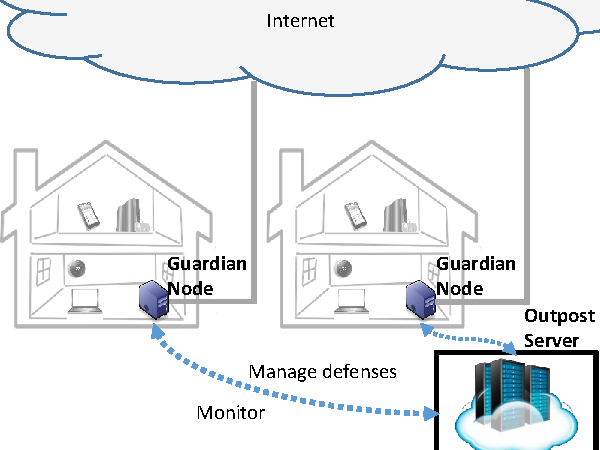
\includegraphics[width=0.95\columnwidth]{figs/highlevel.pdf}
    %\caption{\sysname architecture.}
    %\label{fig:arch}
%\end{figure}
%
%

